\documentclass[a4paper, 15pt]{article}
\usepackage[spanish]{babel}
\usepackage[utf8]{inputenc}
\usepackage{graphicx}
\usepackage{multirow}

\begin{document}
\pagenumbering{gobble}
\begin{titlepage}
   \begin{center}
   \includegraphics[width=6cm]{recursos/logo_UNC}
   
   \Huge
   \textbf{Propuesta de Práctica Profesional Supervisada}
   
   \vspace{0.5cm}
   \LARGE
   Investigación y aprendizaje sobre herramientas de desarrollo en el kernel de FreeBSD

   \vspace{0.5cm}
   \Large
   \underline{\textbf{Alumno:}}
   
   \textbf{Rivero, Franco Fabián \\38111351}
   \vspace{0.2cm}
   
   \underline{\textbf{Tutor:}}
   
   \textbf{Maximiliano Eschoyes}
   
   \vspace{0.5cm}
   
   \textit{Facultad de Ciencias Exactas, Físicas y Naturales}\\
   \textit{Universidad Nacional de Córdoba}\\
   \textit{Cordoba, 2021}
   
   \vspace{1.4cm}
   
   
\includegraphics[width=5cm]{recursos/logo}
\end{center}  
\end{titlepage}
\huge
\textbf{Descripción de actividades}

\vspace{0.4cm}
\large
\begin{flushleft}
Se realizará una investigación sobre FreeBSD, cambios dentro de su kernel, desarrollo de nuevos módulos. Basándome en el proyecto final \textbf{Modelado del planificador a corto plazo con redes de Petri} de los compañeros Nicolas Papp y Tomas Turina se realizara una investigación de las modificaciones hechas. Se dividirá la tarea en algunas etapas para simplificar la complejidad de la tarea.
En una primera etapa se investigará las herramientas a utilizar y lograr preparar el entorno de desarrollo en una máquina virtual. En la segunda parte se buscara automatizar el armado del entorno y buscar herramientas para medir el rendimiento de los distintos planificadores a corto plazo en la plataforma FreeBSD.

\end{flushleft}
\newpage
\begin{flushleft}
\Huge
\textbf{Objetivos}
\vspace{0.7cm}

\huge
\textbf{Objetivos generales}
\vspace{0.4cm}

\large
El estudiante aprenderá sobre tecnologías existentes para el desarrollo en kernel de un sistema operativo, más específicamente en FreeBSD. También adquirirá experiencia en investigación, resolución de problemas y herramientas de virtualización con las tecnologías que se están utilizando hoy en día.

\vspace{0.7cm}
\huge
\textbf{Objetivos específicos}
\vspace{0.4cm}

\large
Proyecto: Investigación y aprendizaje sobre herramientas de desarrollo en el kernel de FreeBSD.

\vspace{0.5cm}
El proyecto a llevar a cabo se divide en objetivos específicos:
\begin{enumerate}
	\item Estudio, aprendizaje e investigación
	\begin{enumerate}
		\item Instalación del sistema operativo FreeBSD en una máquina virtual
		\item Instalación de paquetes y configuración del sistema operativo
		\item Compilación de un kernel de FreeBSD
		\item Encontrar herramientas viables para lograr automatizar y facilitar un entorno para poder compilar FreeBSD
		\item Automatizar la creación de máquinas virtuales de prueba
		\item Encontrar herramientas para poder medir el rendimiento del sistema
		\item Compilar el kernel con los cambios realizados por Nicolas y Tomas.
	\end{enumerate}
	\item Creación de informe sobre el trabajo realizado
	\item Prepararado de presentación y exposición oral de los objetivos cumplidos
\end{enumerate}	
\end{flushleft}
\newpage
\begin{flushleft}
	\Huge
	\textbf{Cronograma de actividades y distribución de carga horaria}
	\vspace{0.7cm}
	
	\large
	La finalización de la PPS se prevé en un lapso de 200 hs. de trabajo, con dedicación mixta con la siguiente distribución:
	
	\large
	\begin{itemize}
		\item \textbf{Tarea 1 (10 hs):} Investigacion sobre el sistema operativo FreeBSD.
		\item \textbf{Tarea 2 (15 hs):} Instalación de FreeBSD en una máquina virtual.
		\item \textbf{Tarea 3 (15 hs):} Configuración de FreeBSD.
		\item \textbf{Tarea 4 (25 hs):} Compilación del kernel dentro de FreeBSD.
		\item \textbf{Tarea 5 (25 hs):} Compilación con un kernel modificado dentro de FreeBSD.
		\item \textbf{Tarea 6 (10 hs):} Investigar sobre herramientas de deployment y automatización
		\item \textbf{Tarea 7 (50 hs):} Automatización de generación de máquinas virtuales
		\item \textbf{Tarea 8 (25 hs):} Análisis de viabilidad de herramientas de profiling 
		\item \textbf{Tarea 9 (25 hs):} Compilacion de kernel con el scheduler modificado para soportar redes de Petri
	\end{itemize}
	\vspace{0.7cm}
	\Large
	\textbf{Diagrama de Gantt}
	\vspace{1cm}

	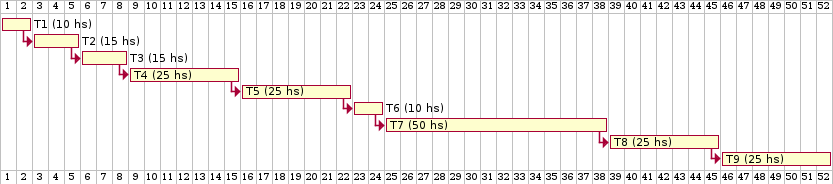
\includegraphics[width=16cm]{recursos/gantt_diagram}
\end{flushleft}


\end{document}